\documentclass[lettersize,journal]{IEEEtran}
% =====================================================================
%  IEEEtran 主文件说明（写给未来的你/合作者看的注释）
% =====================================================================
% 1) 文件结构（推荐的组织方式）
%    - 本文件：KAMMT-trans.tex（主入口，负责：导言区、标题作者信息、整体排版、文末参考文献）
%    - 图像文件：建议统一放到 Figures/ 目录下，例如：Figures/xxx.pdf / .png / .jpg
%    - 参考文献库：references.bib（BibTeX 数据库，文末通过 \bibliography{references.bib} 调用）
%    - 如果正文很长：可把各章节拆到子文件（例如 sections/intro.tex），再在主文件用
%      \input{sections/intro} 或 \include{sections/intro} 组织。
%
% 2) 编译方式（Overleaf）
%    - Overleaf 一般会自动运行（pdfLaTeX + BibTeX + pdfLaTeX + pdfLaTeX）来生成参考文献。
%    - 若你发现引用显示为 [?]：通常是 .bib 没编译成功或 key 不匹配。
%
% 3) 插入图片（graphicx）
%    - 单栏图（IEEE 常用）：
%        \begin{figure}[!t]
%          \centering
%          \includegraphics[width=\linewidth]{Figures/your-figure}
%          \caption{...}
%          \label{fig:your_label}
%        \end{figure}
%      说明：文件扩展名可省略（如 your-figure.png/pdf），LaTeX 会自动选择。
%
%    - 跨双栏大图：用 figure* 环境（你在文中已用到）：
%        \begin{figure*}[!t] ... \end{figure*}
%
%    - 子图（subfig）：
%        \subfloat[子图1]{\includegraphics[width=0.48\linewidth]{Figures/a}}
%        \subfloat[子图2]{\includegraphics[width=0.48\linewidth]{Figures/b}}
%
%    - 图的引用：
%        \ref{fig:your_label} 或（已加载 cleveref）\cref{fig:your_label}
%
% 4) 引用文献（cite + BibTeX）
%    - 文中引用：\cite{key}；多个条目：\cite{key1,key2,key3}
%    - 在 references.bib 里新增/修改条目，确保条目的 key 与 \cite{} 一致。
%    - 文末参考文献：
%        \bibliographystyle{...}
%        \bibliography{references.bib}
%      说明：IEEE 期刊/会议通常使用 IEEEtran 的 bst（例如 IEEEtran/IEEEtranN），
%      你当前用的是 unsrt；如需严格 IEEE 样式，可改为：\bibliographystyle{IEEEtran}
%
% 5) 交叉引用（建议习惯）
%    - 公式：\label{eq:xxx}，文中 \cref{eq:xxx}
%    - 表格：\label{tab:xxx}，文中 \cref{tab:xxx}
%    - 小技巧：label 前缀统一（fig:/tab:/eq:/sec:）能极大降低维护成本。
% =====================================================================

\usepackage{amsmath,amsfonts}
\usepackage{algorithmic}
\usepackage{algorithm}
\usepackage{array}
\usepackage[caption=false,font=normalsize,labelfont=sf,textfont=sf]{subfig}
\usepackage{textcomp}
\usepackage{stfloats}
\usepackage{url}
\usepackage{verbatim}
\usepackage{graphicx}
\usepackage{cleveref}
\usepackage{cite}
\usepackage{booktabs}
% \usepackage{generic}
\usepackage{cite}
\usepackage{multirow}
\usepackage{subfig}
\usepackage{amsmath,amssymb,amsfonts}
\usepackage{cite}
\usepackage{graphicx}
\usepackage{hyperref}
\usepackage[cmyk]{xcolor}
\usepackage{soul, color, xcolor}


\hyphenation{op-tical net-works semi-conduc-tor IEEE-Xplore}
% updated with editorial comments 8/9/2021

\begin{document}

\title{KAMT: Knowledge-aware multi-modal learning based ADRD diagnosis}

\author{IEEE Publication Technology,~\IEEEmembership{Staff,~IEEE,}
        
}

% The paper headers
\markboth{Trans}%
{Author \MakeLowercase{\textit{et al.}}: KAMTT}



\maketitle

\begin{abstract}
        For precision diagnosis, the model performance of deep learning approaches has a over-reliance on sample size and data quality.
        In this case, domain knowledge has played an essential role in enhancing the credibility and reliability of deep learning approaches, especially in precision medicine applications. Neuroimage samples and clinical metadata have been employed to conduct precision diagnostic models for ADRD and cognitive impairment. For the textual modality associated with AD and dementia, the semantic relations between biomedical entities could be applied as domain knowledge to guide the learning of deep neural networks. Under the MML framework, this work proposes the KAMT architecture to enhance prediction accuracy and credibility in ADRD diagnosis.   
        
\end{abstract}

\begin{IEEEkeywords}
	Clinical knowledge, multi-omics integration, ADRD diagnosis.
\end{IEEEkeywords}

\section{Introduction}
\label{sec:introduction}

    \textcolor{blue}{\IEEEPARstart{A}{ssessment} of brain diseases has become an important topic in precision medicine. For neurodegenerative diseases such as Parkinson's disease(PD) and Alzheimer's disease(AD),} multimodal deep learning integrating Electronic Health Records (EHR, containing static demographic backgrounds), Biomarkers (Bio, containing dynamic clinical scales), and 3D-CNN preprocessed Magnetic Resonance Imaging (MRI) has gradually become the mainstream approach. However, when applied to multi-center clinical cohorts with heterogeneous feature distributions, existing purely data-driven models suffer from severe overfitting and performance degradation due to the lack of prior guidance on underlying pathological mechanisms. Furthermore, they heavily rely on numerical and image feature extraction, ignoring the critical semantic associations between biomedical entities in medical records.

    \textcolor{blue}{With efficient representations, the Knowledge-Augmented learning scheme could provide a way to improve the model performance as well as model explainability. It is noted that the quality of knowledge representations determines the prediction accuracy and model generalization ability in precision medicine.} However, directly applying unrefined, large-scale general knowledge graphs to specific diagnostic models introduces overwhelming biological noise, diminishing the model's focus on targeted pathological mechanisms. Conversely, basic graphs built solely from internal diagnostic records suffer from limited data sources and lack deep medical logic support.\textcolor{blue}{Motivated by established works about large-scale biomedical knowledge graphs including SPOKE and PharmKG, this work develops the dementia-specific knowledge graphs by extracting complicated causal relations between biomedical ontology that are associated with brain disease and cognitive decline.}

    \textcolor{blue}{Knowledge-augmented neural network learning architecture is another essential perspective in obtaining reliable predictions} from multimodal data. \textcolor{blue}{With external knowledge, Relational knowledge graphs were constructed to capture causal relations for biomedical entities} that are associated with dementia and cognitive decline. For neurological disorders, essential clinical ontologies such as vascular dynamics and immune regulation have been encoded as the triplets in large-scale biomedical KG.
    \hl{To be specific, which types of biomedical entities were employed. How to focus on vascular dynamics that are abnormal?}

    The main contributions of KAMT architecture were summarized as follows:
	
    \begin{itemize}
        \item High-quality knowledge representations have been extracted and exploited in disease prediction;
        \item Domain knowledge-augmented learning scheme has been proposed to integrate augmented knowledge representations and multi-modal learning.
        \item The positive role of the \textcolor{blue}{clinical knowledge distillation strategy}.
    \end{itemize}


\section{Related Works about Knowledge-guided Learning}

    For neurological disorders, multi-omics integration technology has provided a feasible and effective solution to obtain a comprehensive disease prediction model. However, substantial heterogeneity exists between neuroimage and \hl{transcriptomic} data, which have played a crucial role in precision medicine applications.
    The neuroimaging modality focuses on visual features of the human brains, including the grey and white matter, while the transcriptomic modality captures the molecular changes of disease-specific genes and proteins.
    
    In general, omics data tend to encode microscopic-scale features about human diseases. Among multi-omics data, blood expression data contain transcriptional signatures about immune function and neuroinflammation. Efficient deep neural networks are necessary to obtain biomedically meaningful patterns from blood expression data.
    
\subsection{Multimodal learning based dementia diagnosis}

    \textcolor{blue}{Under the framework of multi-modal learning, neuroimaging and textual modalities have been integrated.}

\subsection{Representation Learning of MRI samples}

    \textcolor{blue}{In feature extraction, two 3D convolutional layers have been employed to analyze neuroimages. The first convolutional layer mainly processes the inherent relations of neuroimages, extracting low-level edge texture information. The second convolutional layer of the 3D-CNN backbone further extracts visual representation from multiple processed features. In this way, the structural features of 3D-MRI samples were extracted and exploited.
    After passing through the activation function and fully connected layer, more comprehensive representations are obtained for subsequent machine learning.}

    
    \subsection{Local Semantic Segmentation of Neuroimages}

    The preprocessing of neuroimages mainly uses detail enhancement based on brain atlas templates, enhancing the important details in brain images, primarily including N4 bias field correction. As a preprocessing technique commonly used for MRI images, bias field correction eliminates the field effects caused by the uneven magnetic fields or radiofrequency fields of the MRI scanner. Through this operation, the whole image does not have noticeable differences in certain areas, thus avoiding noise in subsequent image analysis and processing. The mathematical formula for N4 bias field correction in neuroimage preprocessing is formulated as follows.

    \begin{equation}
        I(x)=J(x)\cdot B(x)+\epsilon(x)
        \label{SemanticAugment}
    \end{equation}

    In Eq.~(\ref{SemanticAugment}), $I(x)$ denotes the observed image intensity, and $B(x)$ represents the real tissue signal intensity. $\epsilon(x)$ is a smooth function corresponding to the bias field. The purpose of semantic augmentation is to estimate and correct the bias field to restore real tissue signals. MR samples have been aligned to be preprocessed with the brain atlas, thus determining the percentile of brain tissue pixels. % to adjust the image intensity range. 
    Furthermore, the grayscale value of the image is adjusted by intensity standardization. To avoid the lack of comparability between neuroimages. Intensity standardization can be expressed by Eq.(\ref{IntensityStandard}).

    \begin{equation}
        I_{norm}(i,j,k)=clip(\frac{I(i,j,k)-P_{p1}}{P_{p99}-P_{p1}},0,1)
        \label{IntensityStandard}
    \end{equation}

    In Eq.(\ref{IntensityStandard}), $I(i,j,k)$ denotes the intensity value of the original image at position $(i,j,k)$, $P_{p1}$ and $P_{p99}$ represent the effective pixel at the $p_1$-th and $p_{99}$-th percentile. The operation $clip(x,0,1)$ clipped $x$ to the range of [0, 1]. 
    
    By applying common anatomical constraints to remove tissue that is not the brain, the signal ratio of gray matter to white matter was controlled to enhance the image symmetry. In the subsequent convolution operation, the texture details of the 3D-MRI samples will be captured and analyzed.

    \subsection{Alignment between MRI-Clinic pairs}

    \textcolor{blue}{Cross-modal interactions were captured by the multimodal Transformer architectures.}
    
\section{Knowledge-Augmented dementia diagnosis}

    \textcolor{blue}{}
    In the precision diagnosis of brain diseases, the primary function of Knowledge Graph Embedding (KGE) is to project the deep semantic information of biomedical entities and relevant relationships into a low-dimensional vector space. 
    
    \textcolor{blue}{Knowledge Graph Embedding (KGE) effectively learns low-rank representations of entities and relations, preserving graph structure and encoding relation semantics by optimizing a training loss that maximizes scores for positive triplets while minimizing those for corrupted triplets. KGE methods, such as TransE, DistMult, ComplEx and RotatE, have shown notable performance in several benchmark tests, but they are often limited to one-hop relations. In large biomedical KGs, relationships between entities are intricate and may involve multihop paths.}
    
    In this case, clinical knowledge representations could be obtained to be injected into multimodal learning. Heterogeneous representations were projected into a specific embedding space. 
    With the DistMult-based translation framework, graph representations of clinical knowledge were constructed to explore the functional relations between biomedical entities about neurodegeneration/dementia, especially from the molecular level. Incorporation of ClinicKG tends to enhance the reliability and accuracy of multimodal learning approaches.

    \begin{figure*}[th]
    	\centering
    	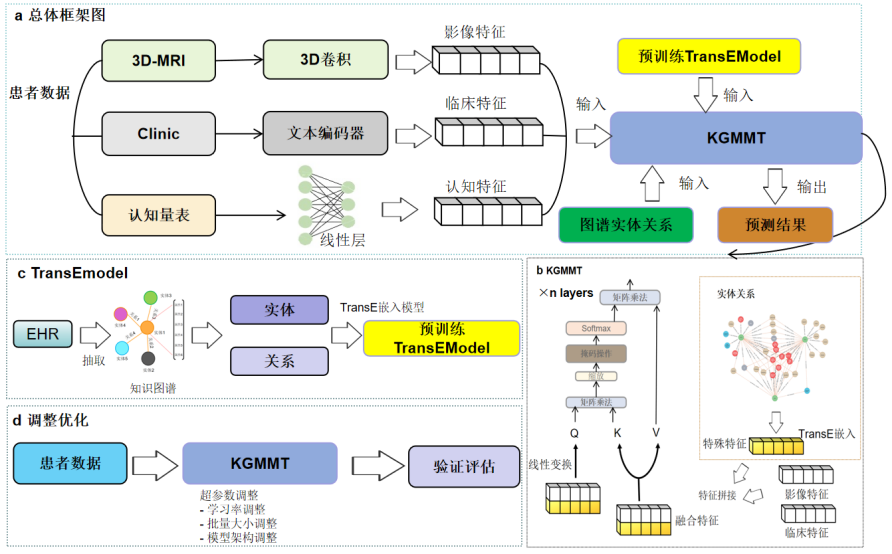
\includegraphics[width=1\linewidth]{Figures/Fig3-FrameworkKAMMT.png}
            \caption{The overview of the multi-modal learning based KAMMT method. Clinical knowledge about neurological disorders has been extracted as graph-structured representations. Graph representations of the constructed ClinicKG have been injected into multi-modal Transformer as constraints to obtain high-credibility predictions about disease states and cognitive dysfunction.}
    	\label{fig5}
    \end{figure*}

    As demonstrated by Fig.\ref{fig5}, the block (A) of the KAMT framework depicts multi-omics data about neurological disorders. A multimodal encoder processes MRI data, clinical metadata, and cognitive scale data separately, representing three different types of common features. A 3D convolutional network has been applied to extract MRI features, while a linear layer is used to process cognitive scale data. Meanwhile, a text encoder is used to process diagnostic information. The encoded features are then processed by the K-guided model using self-attention and cross-attention mechanisms. Section (C) of the framework diagram extracts domain knowledge from tabular-formatted clinic metadata, intending to extract the clinical knowledge graphs. 
    
    The pre-training mechanism of TransE aims to convert prior knowledge into feature vectors. The conventional TransE framework aims to convert biomedical entities and relationships in the clinical knowledge graph extracted from the EHR into low-dimensional embedding vectors, which serve as special vectors. These vectors are subsequently combined with other features to enhance the expressive ability of multimodal networks. For multi-omics data, cross-modal interactions between heterogeneous representations have been captured.
    


\subsection{Construction of Heterogeneous Knowledge Graph}

    To capture latent non-linear associations within multimodal data, this work construct heterogeneous Knowledge Graph (HKG) via a semantic triple-based strategy. We transform structured CSV clinical tables into graph representations and employ the DistMult architecture to project discrete entities and relations into low-dimensional vectors in the continuous latent space.

    \subsubsection{Triples from Clinical Metadata}
    
    `Subject-centric' topology has been adopted to construct the knowledge graph. For the given datasets (ADNI, NACC, AIBL, PPMI), the raw data is defined as a set $D = \{S_1, S_2, \dots, S_N\}$, where each sample $S_i$ contains a sequence of attributes $A = \{a_1, a_2, \dots, a_M\}$.

    In the data table, each non-empty entry was mapped to a semantic triple $(h, r, t)$ based on the following rules:
    
    \begin{itemize}
        \item \textbf{Head Entity ($h$):} Corresponds to the unique identifier of the sample (e.g., \texttt{Subject\_ID} or \texttt{Filename}), serving as the hub node in the graph.
        \item \textbf{Relation ($r$):} Corresponds to the column name (e.g., \texttt{age}, \texttt{apoe}, \texttt{mmse}), defining the semantic edge type.
        \item \textbf{Tail Entity ($t$):} Corresponds to the specific observed value in the cell.
    \end{itemize}

    To eliminate data noise and ensure graph sparsity and accuracy, strict preprocessing logic is executed. The generated set of training triples $\mathcal{T}$ is formally expressed by Eq.(\ref{Eq3}).
    
    \begin{equation}
        \resizebox{0.9\linewidth}{!}{$
        \mathcal{T} = \{ (e_{sub}, r_{attr}, e_{val}) \mid e_{sub} \in \mathcal{E}_{S}, r_{attr} \in \mathcal{R}, e_{val} \in \mathcal{E}_{V}, \text{Val}(e_{sub}, r_{attr}) \neq \text{NaN} \} $}
        \label{Eq3}
    \end{equation}

    where $\mathcal{E}_{S}$ denotes the set of subject entities, $\mathcal{R}$ denotes the set of clinical attribute relations, and $\mathcal{E}_{V}$ denotes the set of attribute value entities. During the preprocessing, the numerical discretization step aims to enhance feature reusability. Continuous variables (e.g., cognitive scores) were rounded to one decimal place, thus converting values into biomedical entities.


    To ensure fair evaluation, the step of Leakage Prevention strictly excluded columns containing final diagnostic labels (e.g., \texttt{NC}, \texttt{MCI}, \texttt{AD}, \texttt{Group}). The graph encodes only objective features such as demographics, genetics, and baseline scores, ensuring that the generated embeddings $\mathbf{e}$ do not contain Ground Truth information.


\subsubsection{DistMult-based Knowledge Embedding}

    \textcolor{blue}{After obtaining structured triples, the DistMult scheme was utilized to obtain biologically meaningful knowledge representations.} 
    As a bilinear diagonal knowledge graph embedding, the DistMult framework has effectively captured symmetric relations with a bilinear form.

    Given a specific triple $(h, r, t)$, the scoring function $f(h, r, t)$ was defined by Eq.(\ref{DistMult}).
    
    \begin{equation}
        f(h, r, t) = \mathbf{h}^T \text{diag}(\mathbf{r}) \mathbf{t} = \sum_{i=0}^{d-1} \mathbf{h}_i \cdot \mathbf{r}_i \cdot \mathbf{t}_i
        \label{DistMult}
    \end{equation}

    where $\mathbf{h}, \mathbf{r}, \mathbf{t} \in \mathbb{R}^d$ represent the $d$-dimensional embeddings of the head, relation, and tail, respectively, and $\text{diag}(\mathbf{r})$ is the diagonal matrix of $\mathbf{r}$. This function aims to maximize scores for valid triples while minimizing them for invalid ones.

    \textcolor{blue}{Furthermore, a stochastic Local Closed World Assumption (SLCWA) has been employed in negative sampling. Early stopping strategy was triggered if the Mean Reciprocal Rank (MRR) on the validation set improved by less than $0.002$ over $10$ consecutive epochs.}
    Upon training completion, the subject node embeddings $\mathbf{e}_{sub}$ are extracted as knowledge-augmented feature inputs for the downstream multimodal classifier.


\subsection{Augmented HKG Representations}

    While the data-driven graph captures statistical regularities within the dataset, it lacks the biological context necessary for understanding regulatory mechanisms for brain diseases. To bridge this gap, we propose a \textit{Hybrid Graph Construction} strategy that anchors patient-specific clinical data to a curated medical knowledge backbone derived from \textcolor{blue}{DementiaHKG}.

\subsubsection{Clinical Knowledge Representations}

    Instead of incorporating the entire large-scale external knowledge graph, which introduces noise, we extract a domain-specific subgraph relevant to neurodegenerative diseases. We define the knowledge backbone $\mathcal{K}_{ext}$ as a set of `Gold Standard' triples:

    \begin{equation}
        \mathcal{K}_{ext} = \{ (h_{concept}, r_{bio}, t_{concept}) \mid h, t \in \mathcal{C}_{\textcolor{blue}{DementiaHKG}} \}
        \label{Eq5}
    \end{equation}

    where $\mathcal{C}_{\textcolor{blue}{DementiaHKG}}$ represents standardized medical concepts (e.g., \texttt{Gene:APOE}, \texttt{Anatomy:Hippocampus}, \texttt{Symptom:Tremor}), and $r_{bio}$ denotes biological relationships (e.g., \texttt{associated\_with}, \texttt{localized\_in}). These triples are manually curated in our implementation to ensure high relevance to AD and PD pathologies.

\subsubsection{Semantic Alignment with External Knowledge}

    To integrate patient data with $\mathcal{K}_{ext}$, we employ a semantic mapping function $\mathcal{M}$ that aligns the column attributes of the clinical CSV files with the concepts in $\mathcal{C}_{\textcolor{blue}{DementiaHKG}}$. For a given attribute column $a_j$ (e.g., \texttt{npiq\_AGIT}), if $\mathcal{M}(a_j) = c_{target} \in \mathcal{C}_{\textcolor{blue}{DementiaHKG}}$, we construct a hierarchical connection path.

    Unlike the direct mapping in the data-driven graph, we introduce an intermediate \textbf{Instance Node} to represent the specific severity or level of a symptom. For a patient $p_i$ having a value $v$ on attribute $a_j$, two coupled triples have been generated:
    
    \begin{align}
        t_{individual} &= (p_i, \texttt{exhibits}, e_{inst}) \\
        t_{conceptual} &= (e_{inst}, \texttt{is\_instance\_of}, c_{target})
        \label{Eq6}
    \end{align}

    where $e_{inst}$ is the instance node formatted as ``$c_{target}\_Level\_v$'' (e.g., \texttt{Tremor\_Level\_2}).

    This hierarchical structure $p_i \to e_{inst} \to c_{target}$ achieves two goals, namely granularity preservation and knowledge anchoring. \textcolor{blue}{In the process of granularity preservation, the node embeddings $e_{inst}$ has preserved the specific feature values, that are associated with the severity of disease symptoms. As for knowledge anchoring, the target node $c_{target}$ served as an anchor, linking sampless exhibiting this symptom to the broader biological network in $\mathcal{K}_{ext}$.}
    
    In this case, the augmented knowledge representation $\mathcal{G}_{aug}$ is the union of the patient-specific instance triples and the external knowledge backbone:
    
    \begin{equation}
        \mathcal{G}_{aug} = \mathcal{T}_{data} \cup \{t_{individual}, t_{conceptual}\} \cup \mathcal{K}_{ext}
    \end{equation}

    The DistMult translation strategy was applied to $\mathcal{G}_{aug}$ to determine knowledge-enhanced embeddings.







\subsection{Knowledge-Guided Multimodal Synergistic Interaction}

Clinical data for brain diseases, such as demographic records (EHR), clinical assessment scales (Bio), and MRI scans, inherently contain high levels of noise and heterogeneity. When analyzing these small patient cohorts, standard data-driven attention mechanisms often overfit to spurious statistical correlations, causing the optimization process to easily trap in local optima. To address this practical challenge, we propose a domain knowledge-guided multimodal collaborative interaction architecture (KAMT).

Rather than relying purely on data frequency, this architecture introduces a modality-aware knowledge retrieval mechanism. It establishes an energy minimization framework grounded in prior constraints at the foundational level. This design effectively translates high-quality medical knowledge into an implicit, dynamic regularization term, which fundamentally regulates the training trajectory of the deep neural networks. The synergistic interaction logic of KAMT, detailing the integration of modality-specific knowledge and the constrained optimization pathway, is systematically illustrated in \cref{fig:KAMT_framework}.

\begin{figure*}[!t]
    \centering
    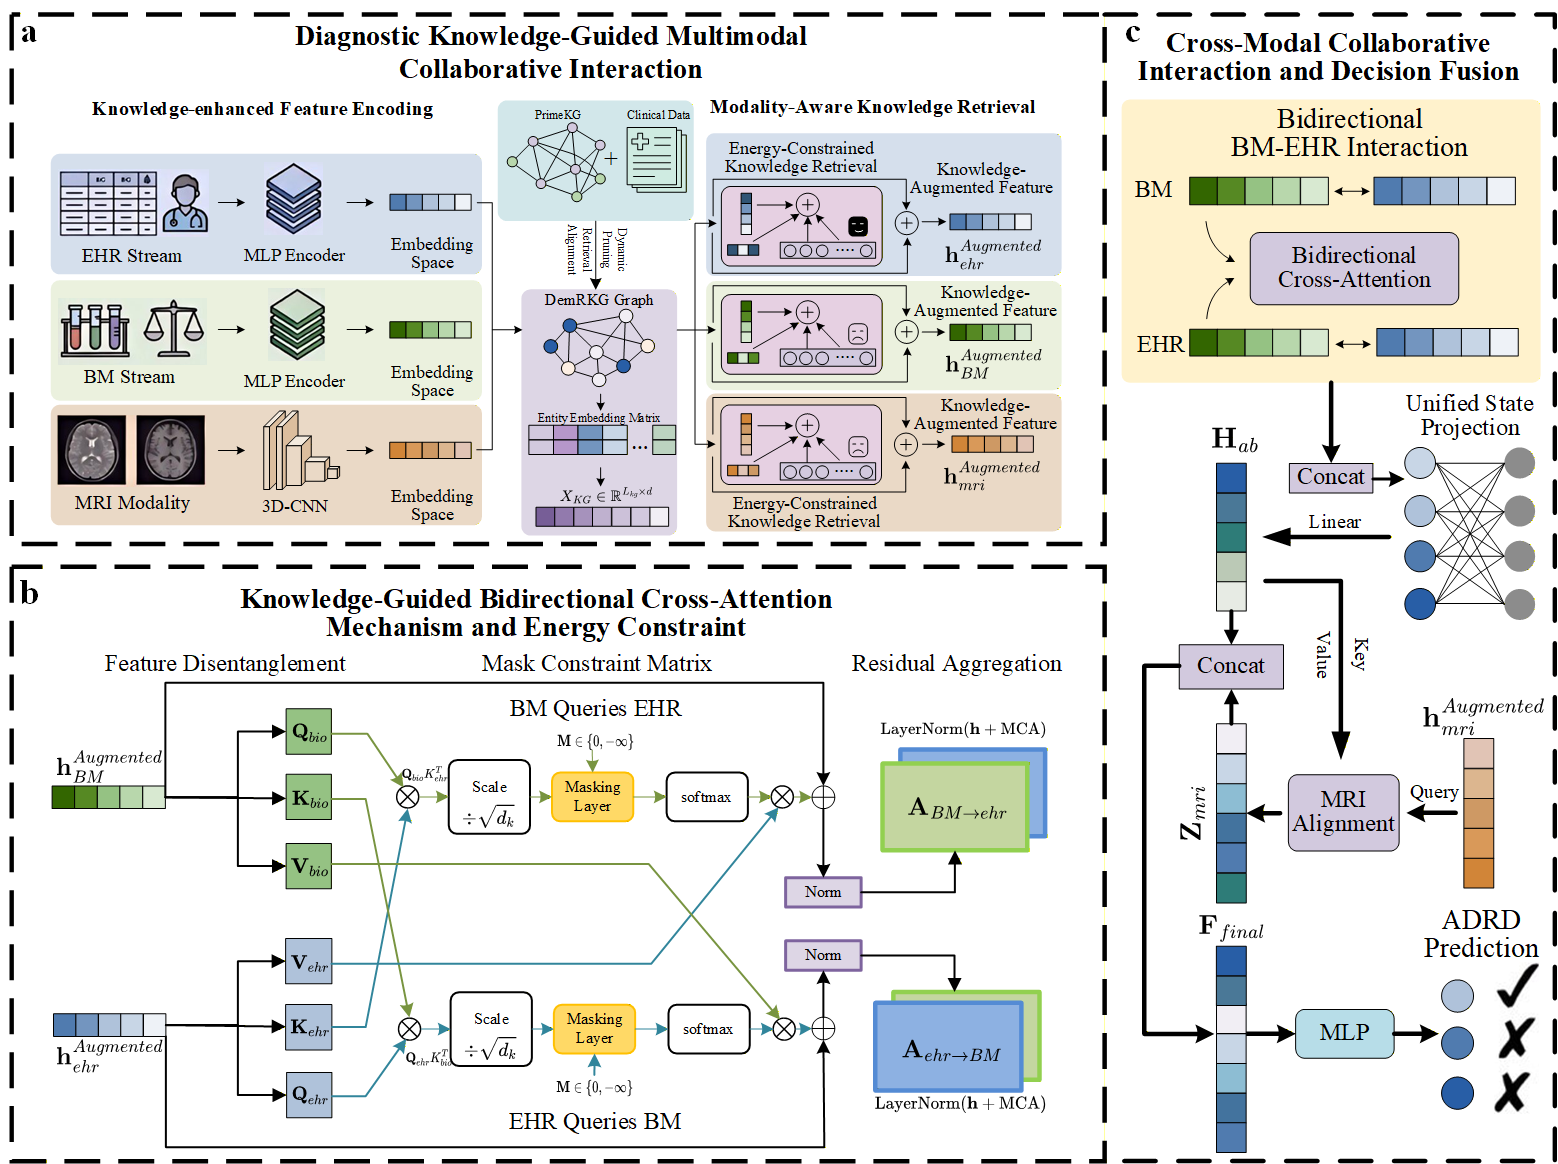
\includegraphics[width=\textwidth]{Figures/KAMT-Trans框架图.png}
    \caption{The overall architecture of the Diagnostic Knowledge-Guided Multimodal Collaborative Interaction (KAMT). (a) Knowledge-Enhanced Feature Encoding and Modality-Aware Knowledge Retrieval: Clinical modalities (EHR, Bio, MRI) are embedded and aligned with corresponding sub-graphs from the medical knowledge graph. (b) Knowledge-Guided Bidirectional Cross-Attention Mechanism and Energy Constraint: A masked cross-attention module integrates the retrieved knowledge, establishing an energy-constrained optimization trajectory. (c) Cross-Modal Collaborative Interaction and Decision Fusion: The extracted low-level health state representations guide the alignment of high-order MRI features, followed by a strict information bottleneck strategy for final ADRD prediction.}
    \label{fig:KAMT_framework}
\end{figure*}

\subsubsection{Dynamic Constraints and Prior Guidance of the Knowledge Graph}

Domain knowledge provides a natural boundary for the feature optimization process. The model maps the raw graph sequences into a continuous space via modality-specific projection layers. This step builds a modality-aware knowledge manifold dictionary $\mathcal{M}_{kg}^{(m)}$:
\begin{equation}
\mathcal{M}_{kg}^{(m)} = \mathrm{span} \{ \mathbf{h}_{kg, m}^{(1)}, \mathbf{h}_{kg, m}^{(2)}, \dots, \mathbf{h}_{kg, m}^{(N)} \} \subset \mathbb{R}^d
\label{eq:manifold_dict}
\end{equation}
Here, $\mathbf{h}_{kg, m}^{(i)}$ represents the semantic vector of the $i$-th graph node under modality $m$. This manifold space strictly bounds the pathological and anatomical relationships among clinical entities.

Within this spatial constraint, the search for the optimal representation $\mathbf{h}_m^*$ of the original feature $\mathbf{h}_m$ is formulated as an energy minimization problem:
\begin{equation}
\mathbf{h}_m^* = \arg\min_{\mathbf{h}} \Big( \| \mathbf{h} - \mathbf{h}_m \|^2 + \lambda \mathcal{D}(\mathbf{h}, \mathcal{M}_{kg}^{(m)}) \Big)
\label{eq:energy_min}
\end{equation}
In this objective function, the first term ensures data fidelity so that the learned features stay true to the actual clinical observations. The second term acts as a knowledge prior penalty, measuring the distance between the feature and the specific knowledge manifold. When dealing with noisy medical environments, this penalty reduces the parameter degrees of freedom, pulling the features back into a medically valid range.

\subsubsection{Modality-Specific Knowledge Retrieval and Feature Enhancement}

Initially, the observed values of each modality are mapped to a unified low-dimensional space $\mathbf{h}_m \in \mathbb{R}^{B \times 1 \times d}$ using independent encoders. Based on the patient's current clinical scale scores, the system activates the relevant medical graph nodes and pads them to a preset maximum sequence length $N$ using zero vectors. Concurrently, it generates a precise Boolean mask matrix $\mathbf{M} \in \{0, -\infty\}^{B\times N}$.

To approximate the energy minimization, the model utilizes a masked multi-head cross-attention mechanism. The mask acts as a crucial operational layer that shields meaningless padded areas, preventing the features from incorrectly drifting towards zero vectors during optimization. The computation for the modality-specific knowledge response $\mathbf{z}_{m}^{kg}$ is given by \cref{eq:knowledge_response}:
\begin{equation}
\mathbf{z}_{m}^{kg} = \mathrm{softmax}\left( \frac{(\mathbf{h}_m \mathbf{W}_m^Q) (\mathbf{H}_{kg}^{(m)} \mathbf{W}_m^K)^\top}{\sqrt{d_k}} + \mathbf{M} \right) (\mathbf{H}_{kg}^{(m)} \mathbf{W}_m^V)
\label{eq:knowledge_response}
\end{equation}
The model then internalizes this knowledge response into the original features using residual connections and layer normalization, creating the enhanced feature $\mathbf{h}_m^{enhanced} = \mathrm{LayerNorm}(\mathbf{h}_m + \mathbf{z}_{m}^{kg})$. This residual flow essentially turns static prior constraints into dynamic nonlinear perturbations, providing a robust foundation for the subsequent modality interactions.

\subsubsection{Knowledge-Guided Text Modality Interaction}

Once the features are infused with graph knowledge, KAMT performs cross-attention between the clinical scales (Bio) and demographic phenotypes (EHR). Because the input features now carry domain knowledge, this interaction is driven by objective medical logic rather than mere data correlation. The enhanced features are projected into Query, Key, and Value spaces, where a Cross-Attention Mechanism (MCA) uncovers implicit links.

Taking the Bio-query-EHR process as an example, the bidirectional computation is detailed in \cref{eq:bidirectional_mca}:
\begin{equation}
\begin{aligned}
\mathbf{A}_{bio \rightarrow ehr} &= \mathrm{LayerNorm}(\mathbf{h}_{bio}^{enhanced} + \mathrm{MCA}(\mathbf{Q}_{bio}, \mathbf{K}_{ehr}, \mathbf{V}_{ehr})) \\
\mathbf{A}_{ehr \rightarrow bio} &= \mathrm{LayerNorm}(\mathbf{h}_{ehr}^{enhanced} + \mathrm{MCA}(\mathbf{Q}_{ehr}, \mathbf{K}_{bio}, \mathbf{V}_{bio}))
\end{aligned}
\label{eq:bidirectional_mca}
\end{equation}
This step serves as a dynamic regularization constraint, limiting the model's search path within the parameter space. The interaction results from both directions are then concatenated and reduced in dimension to extract a unified low-level health state representation $\mathbf{H}_{ab}$.

\subsubsection{Image Alignment and Decision Fusion}

For the image modality, after fusing with its specific graph sub-network, an enhanced query $\mathbf{Q}_{img}$ is generated. KAMT uses the previously extracted health state representation $\mathbf{H}_{ab}$ as both Key and Value to perform a cross-level alignment:
\begin{equation}
\mathbf{Z}_{img} = \mathrm{LayerNorm}(\mathbf{h}_{mri}^{enhanced} + \mathrm{MCA}(\mathbf{Q}_{img}, \mathbf{H}_{ab}, \mathbf{H}_{ab}))
\label{eq:mri_alignment}
\end{equation}

To ensure deep internalization of the medical knowledge, we introduce a strict information bottleneck during the final diagnostic phase. The network intentionally cuts off direct access to the original graph vectors. Instead, it only concatenates the compressed low-level feature $\mathbf{H}_{ab}$ and the high-order image feature $\mathbf{Z}_{img}$:
\begin{equation}
\mathbf{F}_{final} = [ \mathrm{Squeeze}(\mathbf{H}_{ab}) \parallel \mathrm{Squeeze}(\mathbf{Z}_{img}) ]
\label{eq:final_fusion}
\end{equation}
This forced design compels the backpropagation gradients to pass entirely through the preceding cross-attention layers and residual structures. It forces the model to learn the deep semantic associations embedded in the domain knowledge, rather than relying on simple feature concatenation. Finally, the fused feature $\mathbf{F}_{final}$ is processed by a Multi-Layer Perceptron (MLP) for classification, achieving an intelligent, knowledge-guided diagnostic prediction.














\section{Experimental outcomes and analysis}

    In the application of ADRD diagnosis, the performance of the proposed KAMT method and SOTA approaches has been evaluated on four groups of datasets. In the ADNI, PPMI, AIBL and NACC benchmarks, multi-omics data have been selected to conduct the diagnosis for neurological disorders.



\subsection{Dataset Descriptions}


\begin{table}[htbp]
    \centering
    \caption{Statistics and Description of the Evaluated Datasets}
    \label{tab:dataset_statistics}
    \begin{tabular}{llccc}
        \toprule
        \textbf{Dataset} & \textbf{Task} & \textbf{Class} & \textbf{Count} & \textbf{Total} \\
        \midrule
        \multirow{3}{*}{ADNI} & \multirow{3}{*}{3-Class} & NC & 211 & \multirow{3}{*}{837} \\
        & & MCI & 475 & \\
        & & AD & 151 & \\
        \midrule
        \multirow{3}{*}{NACC} & \multirow{3}{*}{3-Class} & NC & 2,116 & \multirow{3}{*}{3,708} \\
        & & MCI & 879 & \\
        & & AD & 713 & \\
        \midrule
        \multirow{3}{*}{AIBL} & \multirow{3}{*}{3-Class} & NC & 358 & \multirow{3}{*}{516} \\
        & & MCI & 86 & \\
        & & AD & 72 & \\
        \midrule
        \multirow{4}{*}{PPMI} & \multirow{4}{*}{4-Class} & Control & 125 & \multirow{4}{*}{409} \\
        & & PD & 132 & \\
        & & SWEDD & 72 & \\
        & & Prodromal & 80 & \\
        \bottomrule
    \end{tabular}
\end{table}







\subsection{Performance Comparison}

\begin{table*}[t]
    \centering
    \caption{Overall performance comparison including Custom KG and \textcolor{blue}{DementiaHKG} on four benchmarks.}
    \label{tab:overall_results_merged}
    \begin{tabular}{llccccc}
        \toprule
        Dataset & Method & Accuracy & Recall & F1-Score & Precision & AUC-ROC \\
        \midrule
        \multirow{5}{*}{ADNI}
            & Bimodal (EHR+MRI) & $0.5687 \pm 0.0079$ & $0.3402 \pm 0.0200$ & $0.2548 \pm 0.0367$ & $0.2235 \pm 0.0917$ & $0.6509 \pm 0.0426$ \\
            & Trimodal (EHR+MRI+BIO) & $0.5723 \pm 0.0107$ & $0.3687 \pm 0.0298$ & $0.3126 \pm 0.0504$ & $0.3418 \pm 0.0955$ & $0.6740 \pm 0.0094$ \\
            & Trimodal+KG (TransE) & $0.5917 \pm 0.0313$ & $0.4875 \pm 0.0396$ & $0.4945 \pm 0.0610$ & $0.5435 \pm 0.0706$ & $0.7189 \pm 0.0425$ \\
            & Trimodal+CustomKG (DistMult) & $0.7521 \pm 0.0166$ & $0.7533 \pm 0.0197$ & $0.7394 \pm 0.0150$ & $0.7332 \pm 0.0249$ & $0.9055 \pm 0.0107$ \\
            & \textbf{Trimodal+\textcolor{blue}{DementiaHKG} (DistMult)} & $\mathbf{0.7985 \pm 0.0132}$ & $\mathbf{0.7734 \pm 0.0189}$ & $\mathbf{0.7767 \pm 0.0145}$ & $\mathbf{0.7835 \pm 0.0169}$ & $\mathbf{0.9164 \pm 0.0070}$ \\
        \midrule
        \multirow{5}{*}{AIBL}
            & Bimodal (EHR+MRI) & $0.6451 \pm 0.0477$ & $0.3239 \pm 0.0289$ & $0.2857 \pm 0.0306$ & $0.2715 \pm 0.0520$ & $0.4753 \pm 0.1080$ \\
            & Trimodal (EHR+MRI+BIO) & $0.7230 \pm 0.0635$ & $0.7226 \pm 0.0644$ & $0.6819 \pm 0.0862$ & $0.7932 \pm 0.0735$ & $0.8478 \pm 0.0632$ \\
            & Trimodal+KG (TransE) & $0.8032 \pm 0.0227$ & $0.6846 \pm 0.0274$ & $0.5999 \pm 0.0525$ & $0.6479 \pm 0.1172$ & $0.9403 \pm 0.0057$ \\
            & Trimodal+CustomKG (DistMult) & $0.8634 \pm 0.0244$ & $0.8305 \pm 0.0805$ & $0.8042 \pm 0.0763$ & $0.8060 \pm 0.0537$ & $0.9446 \pm 0.0215$ \\
            & \textbf{Trimodal+\textcolor{blue}{DementiaHKG} (DistMult)} & $\mathbf{0.9063 \pm 0.0117}$ & $\mathbf{0.9111 \pm 0.0210}$ & $\mathbf{0.8929 \pm 0.0134}$ & $\mathbf{0.8810 \pm 0.0133}$ & $\mathbf{0.9676 \pm 0.0080}$ \\
        \midrule
        \multirow{6}{*}{PPMI}
            & Bimodal (EHR+MRI) & $0.3445 \pm 0.0129$ & $0.2968 \pm 0.0097$ & $0.2600 \pm 0.0110$ & $0.2491 \pm 0.0145$ & $0.5391 \pm 0.0140$ \\
            & Trimodal (EHR+MRI+BIO) & $0.3782 \pm 0.0405$ & $0.3291 \pm 0.0397$ & $0.2676 \pm 0.0241$ & $0.2385 \pm 0.0423$ & $0.5890 \pm 0.0405$ \\
            & Trimodal+KG (TransE) & $0.4862 \pm 0.0667$ & $0.4544 \pm 0.0609$ & $0.4313 \pm 0.0698$ & $0.4536 \pm 0.0814$ & $0.6930 \pm 0.0456$ \\
            & Trimodal+CustomKG & $0.6813 \pm 0.0171$ & $0.6349 \pm 0.0215$ & $0.5868 \pm 0.0363$ & $0.5664 \pm 0.0674$ & $0.8900 \pm 0.0129$ \\
            & Trimodal+\textcolor{blue}{DementiaHKG} & $0.7187 \pm 0.0262$ & $0.6687 \pm 0.0364$ & $0.6519 \pm 0.0517$ & $0.7093 \pm 0.0571$ & $0.8950 \pm 0.0352$ \\
            & \textbf{Trimodal+\textcolor{blue}{DementiaHKG} (Enhanced)} & $\mathbf{0.8231 \pm 0.0212}$ & $\mathbf{0.7875 \pm 0.0233}$ & $\mathbf{0.7975 \pm 0.0256}$ & $\mathbf{0.8309 \pm 0.0274}$ & $\mathbf{0.9252 \pm 0.0133}$ \\
        \midrule
        \multirow{5}{*}{NACC}
            & Bimodal (EHR+MRI) & $0.5767 \pm 0.0219$ & $0.3713 \pm 0.0809$ & $0.2870 \pm 0.0835$ & $0.2455 \pm 0.0833$ & $0.6604 \pm 0.0754$ \\
            & Trimodal (EHR+MRI+BIO) & $0.6428 \pm 0.0101$ & $0.4986 \pm 0.0148$ & $0.4799 \pm 0.0160$ & $0.5484 \pm 0.0402$ & $0.6572 \pm 0.0083$ \\
            & Trimodal+KG (TransE) & $0.6711 \pm 0.0054$ & $0.5316 \pm 0.0051$ & $0.4868 \pm 0.0111$ & $0.5663 \pm 0.1001$ & $0.7421 \pm 0.0041$ \\
            & Trimodal+CustomKG (DistMult) & $0.7933 \pm 0.0156$ & $0.7268 \pm 0.0310$ & $0.7322 \pm 0.0252$ & $0.7487 \pm 0.0130$ & $0.9165 \pm 0.0160$ \\
            & \textbf{Trimodal+\textcolor{blue}{DementiaHKG} (DistMult)} & $\mathbf{0.8165 \pm 0.0050}$ & $\mathbf{0.7698 \pm 0.0124}$ & $\mathbf{0.7677 \pm 0.0078}$ & $\mathbf{0.7680 \pm 0.0066}$ & $\mathbf{0.9325 \pm 0.0036}$ \\
        \bottomrule
    \end{tabular}
\end{table*}

Based on the ADNI, PPMI, AIBL, and NACC benchmarks, the performance of various methods has been evaluated and compared in Table \ref{tab:overall_results_merged}. The experimental results clearly validate the three core hypotheses of this study. First, a significant performance gap exists between purely data-driven models and knowledge-guided paradigms. As observed in the PPMI dataset, the baseline Trimodal (EHR+MRI+BIO) model only achieves an F1-Score of $0.2676 \pm 0.0241$. This verifies our hypothesis: existing multimodal learning (MML) networks that purely adopt joint learning and information fusion represent an extensive "stacking" technological paradigm, relying solely on expanding information volume to improve performance. Such an approach struggles to fully bridge the semantic gap between clinical manifestations and underlying pathology. Conversely, the comprehensive metric leaps achieved after introducing knowledge graphs demonstrate that knowledge and data possess an inherent complementarity. They can cooperate perfectly within the MM Transformer architecture, thereby fundamentally improving the reliability and accuracy of disease prediction and diagnosis.

Furthermore, the experimental data highlights the necessity of external knowledge refinement. Although the internally constructed CustomKG yields certain improvements, the DementiaHKG strategy, which introduces large-scale external knowledge bases, achieves substantial growth across all metrics (e.g., reaching an accuracy of $0.8165 \pm 0.0050$ on the NACC dataset), comprehensively surpassing CustomKG. This substantiates our hypothesis: external knowledge bases (such as PrimeKG) significantly outperform the internal CustomKG in both knowledge breadth and depth. Because external biomedical knowledge is often intricate and cluttered, direct application makes it difficult to exert its effectiveness and may be slightly inferior in alignment with downstream tasks. However, the proposed knowledge refinement scheme successfully filters out useless parts, retaining only the components that closely align with the downstream clinical scenario.

Finally, the comparison of embedding algorithms underscores the critical importance of spatial representation matching. Controlling for identical multimodal inputs, models employing DistMult consistently outperform TransE-based models in processing the complex semantics of medical knowledge. For instance, in the AIBL dataset, the accuracy of the DistMult-based model jumps to $0.9063 \pm 0.0117$, significantly higher than the $0.8032 \pm 0.0227$ achieved by TransE. This confirms our hypothesis: compared to TransE, the DistMult knowledge embedding method is more suitable for solving the considered diagnostic scenarios. It can highly adapt to the intrinsic characteristics and distribution patterns of tabular data like Clinical Metadata, effectively analyze the causal relationships between entities such as blood pressure and blood lipids, and provide precise profiling of patients' brain health and dementia risks. The confirmation of these macroscopic experimental phenomena lays a solid foundation for the subsequent in-depth exploration of DementiaHKG's construction, refinement mechanisms, and intrinsic computational logic.
















    
    Evaluation metrics obtained by the proposed KAMMT method demonstrate that our proposed method significantly outperforms traditional baselines and SOTA models.

    \textbf{1. Universal Improvement in Training Stability:}
    A critical observation across selected benchmarks is the stark contrast in training dynamics. As visualized in our training curves (e.g., Loss and AUC), baseline models (Bimodal/Trimodal without KG) frequently exhibited oscillatory loss patterns and failed to reach optimal convergence, likely due to the non-convex nature of the sparse multimodal feature space. In contrast, the introduction of KG embeddings (DistMult/\textcolor{blue}{DementiaHKG}) acted as a stabilizer, enabling rapid and smooth convergence in all tasks. This suggests that structured knowledge is not merely an auxiliary feature but a necessary condition for effective optimization in small-sample medical contexts.

\textbf{2. Overcoming the Limitations of Shallow Fusion:}

    Traditional fusion approaches (concatenation) failed to capture complex non-linear interactions, particularly in the challenging \textbf{PPMI} dataset, where the Bimodal baseline achieved an accuracy of only $0.3168$. Our method improves this to $0.7123$, demonstrating that structured knowledge representation is critical for establishing effective decision boundaries.


\subsection{Construction and Refinement of the Diagnostic Knowledge Graph DementiaHKG}

The construction of DementiaHKG strictly adheres to a rigorous academic paradigm: extracting specific brain disease domain knowledge from massive generic biomedical databases, and subsequently embedding heterogeneous multimodal data into a unified low-dimensional vector space. During the domain-adaptive biological skeleton extraction phase, the experiment employed a top-down knowledge distillation strategy based on PrimeKG, identifying the \textcolor{blue}{selection and characterization of knowledge representations} as the core breakthrough point. To mitigate the noise inherent in generic graphs, the system first utilized \textcolor{blue}{anatomical anchors} (such as the substantia nigra and striatum targeted in the Parkinson's disease extraction) as key elements for directional filtering, forcibly removing redundant anatomical nodes that have no direct association with brain diseases. More importantly, the system explicitly constructed representations for metabolic comorbidity mechanisms, utilizing \textcolor{blue}{clinical history such as hypertension, high cholesterol, and diabetes} as the metabolic foundation within the high-dimensional semantic space, and forcibly extracted corresponding subgraphs for insulin, blood glucose, and lipid signaling pathways.

After establishing the anchors, the algorithm automatically identified orthologous genes connecting clinical symptoms with metabolic nodes, and supplemented them with Protein-Protein Interaction (PPI) edges. \textcolor{blue}{To control the graph over-densification caused by scale-free network characteristics, the experiment implemented a PPI pruning algorithm penalized by node degree constraints.} Given the original gene interaction subgraph, let $deg(v)$ denote the degree of node $v$ within this network, and let $\tau$ be the degree truncation threshold. The retained skeletal edge set after pruning is strictly constrained as:
\begin{equation}
\mathcal{T}_{ppi}^* = \{(h, r_{ppi}, t) \mid \max(deg(h), deg(t)) \le \tau\}
\label{eq:ppi_pruning_rule}
\end{equation}
Taking the greedy pruning strategy with $\tau=5$ as an example, \textcolor{blue}{during the construction of the NACC graph, this algorithm drastically reduced the redundant full-scale PPI network containing 59,888 edges to merely 11,425 skeletal edges; similarly, 1,443 core connections were refined in the PPMI construction.} This process dramatically suppressed the explosion of hub nodes while ensuring physical connectivity. Subsequently, the graph entered the entity instantiation phase for multimodal clinical data. The system not only employed hard-coding to use the APOE gene carrier status as a physical bridge directly connecting patients to core disease nodes, but also \textcolor{blue}{adopted a partial order mapping rule to transform discrete scores such as MDS-UPDRS into hierarchical nodes with directed rank constraints (e.g., $\text{Lv1} \prec \text{Lv2}$).} Ultimately, \textcolor{blue}{by utilizing connected component analysis to prune invalid dangling networks}, the system ensured the accessibility of every phenotypic node to the underlying biological mechanisms.



\subsubsection{Core Advantage Analysis of DementiaHKG over CustomKG}

Compared to CustomKG, which only extracts internal observational co-occurrence patterns, DementiaHKG, by introducing external biomedical priors, demonstrates disruptive advantages in graph scale, semantic quality, and reasoning logic. First and foremost, \textcolor{blue}{DementiaHKG achieved explosive growth in node scale by introducing genes, pathways, and protein interaction networks from PrimeKG.} This strategy thoroughly dismantled the inherent sparsity dilemma of small-sample medical datasets. For instance, constrained by the clinical cohort size, the number of nodes for PPMI in CustomKG was a mere 438; however, \textcolor{blue}{in DementiaHKG, it surged to 10,096 (a more than 20-fold increase).} This strategy of "enveloping" a small number of clinical features with a massive volume of external knowledge nodes successfully embedded discrete observational results into a high-dimensional, dense biological semantic space. Secondly, the evolution of graph relations reflects an exceptional \textcolor{blue}{semantic normalization} effect. Despite the explosive growth in node scale, \textcolor{blue}{the number of relation types for PPMI paradoxically plummeted from 81 in CustomKG to 20.} This is attributed to the fact that the graph construction abandoned the rigid mapping of raw CSV headers, achieving unified alignment at a standardized ontology layer.

Crucially, the emergence of pathological bridges marks the model's \textcolor{blue}{logical leap from "explicit classification" to "implicit reasoning."} In the AIBL dataset, CustomKG strictly zeroed out diagnostic relations to prevent data leakage; in DementiaHKG, however, owing to the precise characterization of representations mentioned above, \textcolor{blue}{the graph successfully spawned 378 implicit pathological bridge edges.} This structural breakthrough freed the black-box model from relying on rote-memorized labels, equipping it with the ability to infer disease risk through pathogenic pathways, thereby endowing the prediction results with invaluable biological interpretability.

\subsubsection{Efficacy of Knowledge Representation Learning and Multimodal Fusion}

    Experimental results of the multimodal classification task indicate that \textcolor{blue}{the knowledge embedding of DementiaHKG achieved immense success. The dramatic leap in downstream performance is merely a surface-level manifestation; one of the intrinsic reasons is the study's decisive adoption of the DistMult method for processing knowledge representation, which significantly reduced feature redundancy and improved computational efficiency, thereby ensuring that the multimodal AI model successfully learned and internalized the deep biological knowledge contained within DementiaHKG.}

From a computational mechanism perspective, DistMult discards the complex translational space assumptions of TransE, quantifies the plausibility of triplets via a bilinear scoring function, and ingeniously constrains the relation matrix to be strictly diagonal $W_r = \text{diag}(w_r)$. This built-in diagonalization constraint reduces the parameter complexity of relations from $\mathcal{O}(d^2)$ to $\mathcal{O}(d)$, which not only effectively controls the risk of overfitting on sparse medical data but also perfectly matches the abundant symmetrical associations present in PPI networks. Driven by the Margin Ranking Loss, true medical facts and random noise are forcibly separated in the 128-dimensional continuous space.

Empirical data provides solid evidence for this theoretical advantage. In the highly complex PPMI dataset, the F1-Score of the baseline Trimodal fusion was only 0.2676; \textcolor{blue}{when graph features based on TransE were introduced, the F1-Score only slightly increased to 0.4313} due to parameter redundancy and inadequate capture of symmetrical relations. However, \textcolor{blue}{when the "Trimodal+DementiaHKG (Enhanced)" strategy combined with DistMult representation was applied, the accuracy skyrocketed to 0.8231, the F1-Score reached 0.7975, and the AUC-ROC peaked at 0.9252.} \textcolor{blue}{Similarly, the accuracy for the AIBL dataset surged from the TransE baseline of 0.8032 to 0.9063 after introducing DistMult representations.} This series of highly consistent metric leaps fully proves that the combination of the low-redundancy, high-efficiency DistMult representation learning strategy with the high-density DementiaHKG biological priors has successfully constructed an impenetrable feature foundation for multimodal diagnostic models.




\subsection{Ablation Study}


\begin{table*}[h]
    \centering
    \caption{Ablation study results on ADNI and NACC datasets. A, B, C, and D represent EHR, MRI, Tensor, and \textcolor{blue}{DementiaHKG} modules, respectively.}
    \resizebox{\textwidth}{!}{%
    \begin{tabular}{c c c c | c c c c c | c c c c c}
    \toprule
    \multicolumn{4}{c|}{\textbf{Modules}} & \multicolumn{5}{c|}{\textbf{ADNI}} & \multicolumn{5}{c}{\textbf{NACC}} \\
    \cmidrule(r){1-4} \cmidrule(lr){5-9} \cmidrule(l){10-14}
    A & B & C & D & ACC & Recall & F1-Score & Precision & AUC & ACC & Recall & F1-Score & Precision & AUC \\
    (EHR) & (MRI) & (Tensor) & (KG) & & & & & & & & & & \\
    \midrule
    % w/o KG (A+B+C)
    \checkmark & \checkmark & \checkmark & & 
    $0.5910 \pm 0.0145$ & $0.4630 \pm 0.0128$ & $0.4710 \pm 0.0161$ & $0.5757 \pm 0.0342$ & $0.7549 \pm 0.0132$ & 
    $0.7296 \pm 0.0015$ & $0.6307 \pm 0.0069$ & $0.6353 \pm 0.0105$ & $0.6622 \pm 0.0064$ & $0.8657 \pm 0.0018$ \\
    
    % w/o Tensor (A+B+D)
    \checkmark & \checkmark & & \checkmark & 
    $0.7612 \pm 0.0195$ & $0.7910 \pm 0.0166$ & $0.7545 \pm 0.0147$ & $0.7405 \pm 0.0186$ & $0.9020 \pm 0.0107$ & 
    $0.7599 \pm 0.0111$ & $0.6863 \pm 0.0196$ & $0.6918 \pm 0.0181$ & $0.7012 \pm 0.0165$ & $0.8865 \pm 0.0046$ \\
    
    % w/o MRI (A+C+D)
    \checkmark & & \checkmark & \checkmark & 
    $0.7537 \pm 0.0245$ & $0.7315 \pm 0.0336$ & $0.7297 \pm 0.0283$ & $0.7353 \pm 0.0282$ & $0.8966 \pm 0.0144$ & 
    $0.7926 \pm 0.0064$ & $0.7282 \pm 0.0095$ & $0.7385 \pm 0.0095$ & $0.7529 \pm 0.0148$ & $0.9135 \pm 0.0016$ \\
    
    % w/o EHR (B+C+D)
    & \checkmark & \checkmark & \checkmark & 
    $0.7716 \pm 0.0154$ & $0.7532 \pm 0.0215$ & $0.7499 \pm 0.0170$ & $0.7506 \pm 0.0199$ & $0.9038 \pm 0.0062$ & 
    $0.7832 \pm 0.0099$ & $0.7184 \pm 0.0158$ & $0.7279 \pm 0.0134$ & $0.7419 \pm 0.0105$ & $0.9065 \pm 0.0037$ \\
    
    % Full method (A+B+C+D)
    \checkmark & \checkmark & \checkmark & \checkmark & 
    $\mathbf{0.7985 \pm 0.0132}$ & $\mathbf{0.7734 \pm 0.0189}$ & $\mathbf{0.7767 \pm 0.0145}$ & $\mathbf{0.7835 \pm 0.0169}$ & $\mathbf{0.9164 \pm 0.0070}$ & 
    $\mathbf{0.8165 \pm 0.0050}$ & $\mathbf{0.7698 \pm 0.0124}$ & $\mathbf{0.7677 \pm 0.0078}$ & $\mathbf{0.7680 \pm 0.0066}$ & $\mathbf{0.9325 \pm 0.0036}$ \\
    \bottomrule
    \end{tabular}
    }
    \label{tab:ablation_adni_nacc}
\end{table*}

\begin{table*}[h]
    \centering
    \caption{Ablation study results on PPMI and AIBL datasets. A, B, C, and D represent EHR, MRI, Tensor, and \textcolor{blue}{DementiaHKG} modules, respectively. The results are reported as Mean $\pm$ Std.}
    \resizebox{\textwidth}{!}{%
    \begin{tabular}{c c c c | c c c c c | c c c c c}
    \toprule
    \multicolumn{4}{c|}{\textbf{Modules}} & \multicolumn{5}{c|}{\textbf{PPMI}} & \multicolumn{5}{c}{\textbf{AIBL}} \\
    \cmidrule(r){1-4} \cmidrule(lr){5-9} \cmidrule(l){10-14}
    A & B & C & D & ACC & Recall & F1-Score & Precision & AUC & ACC & Recall & F1-Score & Precision & AUC \\
    (EHR) & (MRI) & (Tensor) & (KG) & & & & & & & & & & \\
    \midrule
    % w/o KG (A+B+C)
    \checkmark & \checkmark & \checkmark & & 
    $0.6492 \pm 0.0500$ & $0.6027 \pm 0.0400$ & $0.5910 \pm 0.0422$ & $0.6385 \pm 0.0553$ & $0.8217 \pm 0.0305$ & 
    $0.8747 \pm 0.0164$ & $0.8788 \pm 0.0121$ & $0.8597 \pm 0.0145$ & $0.8479 \pm 0.0162$ & $0.9458 \pm 0.0110$ \\
    
    % w/o Tensor (A+B+D)
    \checkmark & \checkmark & & \checkmark & 
    $0.6585 \pm 0.0179$ & $0.6013 \pm 0.0210$ & $0.5933 \pm 0.0212$ & $0.6481 \pm 0.0140$ & $0.8725 \pm 0.0319$ & 
    $0.7470 \pm 0.0590$ & $0.5814 \pm 0.1178$ & $0.5475 \pm 0.1035$ & $0.5546 \pm 0.1116$ & $0.8062 \pm 0.0754$ \\
    
    % w/o MRI (A+C+D)
    \checkmark & & \checkmark & \checkmark & 
    $0.6708 \pm 0.0396$ & $0.6075 \pm 0.0445$ & $0.6008 \pm 0.0477$ & $0.6703 \pm 0.0370$ & $0.8645 \pm 0.0320$ & 
    $0.8458 \pm 0.0696$ & $0.8043 \pm 0.1157$ & $0.7879 \pm 0.1123$ & $0.7815 \pm 0.1030$ & $0.9195 \pm 0.0783$ \\
    
    % w/o EHR (B+C+D)
    & \checkmark & \checkmark & \checkmark & 
    $0.6708 \pm 0.0250$ & $0.6105 \pm 0.0357$ & $0.5996 \pm 0.0410$ & $0.6441 \pm 0.0417$ & $0.8857 \pm 0.0261$ & 
    $0.8627 \pm 0.0223$ & $0.8442 \pm 0.0577$ & $0.8140 \pm 0.0685$ & $0.7996 \pm 0.0632$ & $0.9501 \pm 0.0126$ \\
    
    % Full method (A+B+C+D)
    \checkmark & \checkmark & \checkmark & \checkmark & 
    $\mathbf{0.8231 \pm 0.0212}$ & $\mathbf{0.7875 \pm 0.0233}$ & $\mathbf{0.7975 \pm 0.0256}$ & $\mathbf{0.8309 \pm 0.0274}$ & $\mathbf{0.9252 \pm 0.0133}$ & 
    $\mathbf{0.9063 \pm 0.0117}$ & $\mathbf{0.9111 \pm 0.0210}$ & $\mathbf{0.8929 \pm 0.0134}$ & $\mathbf{0.8810 \pm 0.0133}$ & $\mathbf{0.9676 \pm 0.0080}$ \\
    \bottomrule
    \end{tabular}%
    }
    \label{tab:ablation_ppmi_aibl}
\end{table*}

\subsection{Efficiency of Augmented Knowledge}

    \textcolor{blue}{The custom KG was obtained by the DistMult-based KGE method, while the DemRKG corresponds to the situation of augmented graph representations.}


    \begin{table*}[t]
        \centering
        \caption{Performance comparison between the Custom KG and \textcolor{blue}{DementiaHKG} on four benchmarks. The results are reported as Mean $\pm$ Std.}
        \label{tab:\textcolor{blue}{DementiaHKG}_comparison}
        \begin{tabular}{llccccc}
            \toprule
            Dataset & Method & Accuracy & Recall & F1-Score & Precision & AUC-ROC \\
            \midrule
            \multirow{2}{*}{ADNI}
                & DistMult (Ours) & $0.8370 \pm 0.0334$ & $0.8073 \pm 0.0379$ & $0.8176 \pm 0.0386$ & $0.8444 \pm 0.0458$ & $0.8560 \pm 0.0133$ \\
                & \textcolor{blue}{DementiaHKG} & $\mathbf{0.8632 \pm 0.0252}$ & $\mathbf{0.8494 \pm 0.0336}$ & $\mathbf{0.8500 \pm 0.0294}$ & $\mathbf{0.8574 \pm 0.0224}$ & $\mathbf{0.8663 \pm 0.0108}$ \\
            \midrule
            \multirow{2}{*}{PPMI}
                & DistMult (Ours) & $0.7123 \pm 0.0179$ & $0.6660 \pm 0.0251$ & $0.6409 \pm 0.0473$ & $0.6482 \pm 0.0674$ & $0.8924 \pm 0.0132$ \\
                & \textcolor{blue}{DementiaHKG} & $\mathbf{0.8188 \pm 0.0401}$ & $\mathbf{0.7978 \pm 0.0483}$ & $\mathbf{0.7961 \pm 0.0463}$ & $\mathbf{0.8217 \pm 0.0469}$ & $\mathbf{0.9634 \pm 0.0089}$ \\
            \midrule
            \multirow{2}{*}{AIBL}
                & DistMult (Ours) & $0.9009 \pm 0.0384$ & $0.8971 \pm 0.0450$ & $0.8753 \pm 0.0498$ & $0.8660 \pm 0.0558$ & $0.9780 \pm 0.0133$ \\
                & \textcolor{blue}{DementiaHKG} & -- & -- & -- & -- & -- \\
            \midrule
            \multirow{2}{*}{NACC}
                & DistMult (Ours) & $0.7571 \pm 0.0427$ & $0.6353 \pm 0.0776$ & $0.6404 \pm 0.0818$ & $0.6622 \pm 0.0805$ & $0.8088 \pm 0.0298$ \\
                & \textcolor{blue}{DementiaHKG} & $\mathbf{0.8080 \pm 0.0366}$ & $\mathbf{0.7345 \pm 0.0556}$ & $\mathbf{0.7247 \pm 0.0503}$ & $\mathbf{0.7316 \pm 0.0494}$ & $\mathbf{0.8169 \pm 0.0210}$ \\
            \bottomrule
        \end{tabular}
    \end{table*}


\subsection{Investigation of Clinical Knowledge Representations}

    Table \ref{tab:\textcolor{blue}{DementiaHKG}_comparison} shows that \textcolor{blue}{DementiaHKG} leads to a secondary leap in performance. Based on the universal convergence improvements observed, we identify the following core mechanisms:

    \subsubsection{Stabilization of Optimization Landscape (Global Mechanism)}
    
    The primary contribution of the \textcolor{blue}{KGE learning} is its role as a powerful \textbf{Regularizer}. In medical multimodal learning, the feature space is often high-dimensional yet sparse, creating a highly volatile loss landscape. The injection of pre-trained KG embeddings (DistMult/\textcolor{blue}{DementiaHKG}) provides a stable ``skeleton'' (manifold) for the feature space. This significantly reduces the search space for the Multimodal Transformer, ensuring consistent convergence across all datasets (ADNI, PPMI, NACC), preventing the model from collapsing into random guessing.

\subsubsection{Semantic Anchoring Effect}

    Pure data-driven models treat clinical attributes as isolated symbols. By anchoring attributes (e.g., \texttt{upd2315a}) to standardized entities in \textcolor{blue}{DementiaHKG} (e.g., \texttt{Symptom:Rest\_Tremor}), the model acquires a clear \textbf{Inductive Bias}. This ``God's eye view'' acts as a navigational aid, guiding the gradient descent towards biologically meaningful solutions.

    The \textbf{Hierarchical Instantiation Strategy} ($\text{Patient} \to \text{Level} \to \text{Concept}$) bridges the gap between samples. It ensures that patients with varying symptom severities are drawn closer in the embedding space through shared parent concepts, effectively mitigating the overfitting issues common in small-sample medical data.



    


\section{Discussion}
    

\section{Data availability}

    \textcolor{blue}{The Parkinson’s Progression Markers Initiative (PPMI, http://www.ppmi-info.org/) database and the Parkinson’s Disease Biomarkers Program (PDBP, https://pdbp.ninds.nih.gov/) database used in this study are both accessible through AMP-PD (https://amp-pd.org/). To access clinical and omics data at the AMP-PD Tier 2 level, users are required to complete a data use agreement and submit an online application.}
	

\section*{Code availability}

	This M$^2$STGAT method is implemented in Python and available in Github (https://github.com/ZJ-BMDmining/M2DGAT).


    
\section*{Acknowledgment}

	This work is sponsored by National Natural Science Foundation of China(62302455, 62172369), Special Support Plan for High-level Talents in Zhejiang Province(2021R52019) and Natural Science Foundation of Zhejiang Province, China(LQ24F030007).
	
	

%\section*{References}
\bibliographystyle{unsrt}
\bibliography{references.bib}




\vfill

\end{document}


